\documentclass{article}
\usepackage[utf8]{inputenc}
\usepackage{amsmath}
\usepackage{amssymb}
\usepackage{graphicx}
\usepackage[margin = 1 in]{geometry}



\title{CS5220: Matrix Multiply Project}
\author{Junyoung Lim, Max Ruth, Arjun Sharma}
\date{October 5, 2020}

\begin{document}

\maketitle

\section{Introduction}
We have tried a variety of ways to optimize matrix-matrix multiplication and are able to improve upon the basic algorithm approximately by a factor of three (64\_block vs. basic in figure \ref{fig:timing_methods}). The best optimized case we have obtained achieves only about 35-40\% as efficient as BLAS algorithm (64\_block vs. blas in figure \ref{fig:timing_methods}).

\begin{figure}[h!]
	\centering
	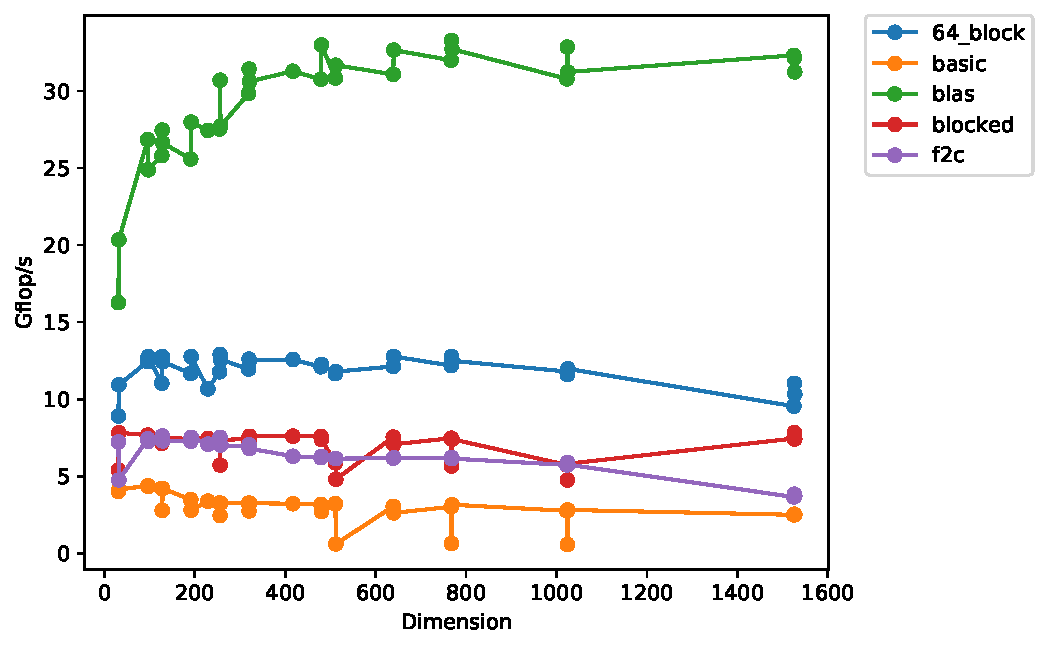
\includegraphics[width=0.8\columnwidth]{timing_methods.pdf}
	\caption{Flop rates for the given f2c, blocked, blas and basic algorithm compared with the our best algorithm, 64\_block.}
	\label{fig:timing_methods}
\end{figure}

In the rest of the report describe the incremental steps that lead us to the 64\_block algorithm. 

References: 

https://stackoverflow.com/questions/38190006/matrix-multiplication-why-non-blocked-outperforms-blocked




\section{Discussion: Compilation Details}
The simplest design decisions that we made were on the compiler side. We used the GCC 8.3.0 compiler that was downloaded by default in the \texttt{build-essential} package. The three flags that we used for the compilation are the following:
\begin{itemize}
	\item \texttt{-O3} --- Enable more aggressive optimization than the flag \texttt{-O2} used by default. 
	\item \texttt{-ffast-math} --- Allows the compiler to reorder operations that may not actually be associative. We did not see a dramatic increase in the error of the result using this flag, although there would be a chance for that when floating point operations are seen as associative. Perhaps for more pathological matrix examples, we might have to worry about this flag.
	\item \texttt{-march=native} --- Optimizes the code for the specific machine architecture. When running on a desktop with the flag \texttt{-fopt-info-vec}, adding \texttt{-march=native} changed the vectorization from 16 bytes to 32 bytes wherever possible - allowing a potential doubling of the computation speed.
\end{itemize}

Of course, there are likely many more compiler options that could have been considered. We did not experiment with the CLang, gfortran, or Intel compilers. From the 


\section{Discussion: the Inner Kernel}
Plot: restrict vs. not restrict

\subsection{The \texttt{restrict} Keyword}
\begin{figure}[h!]
    \centering
    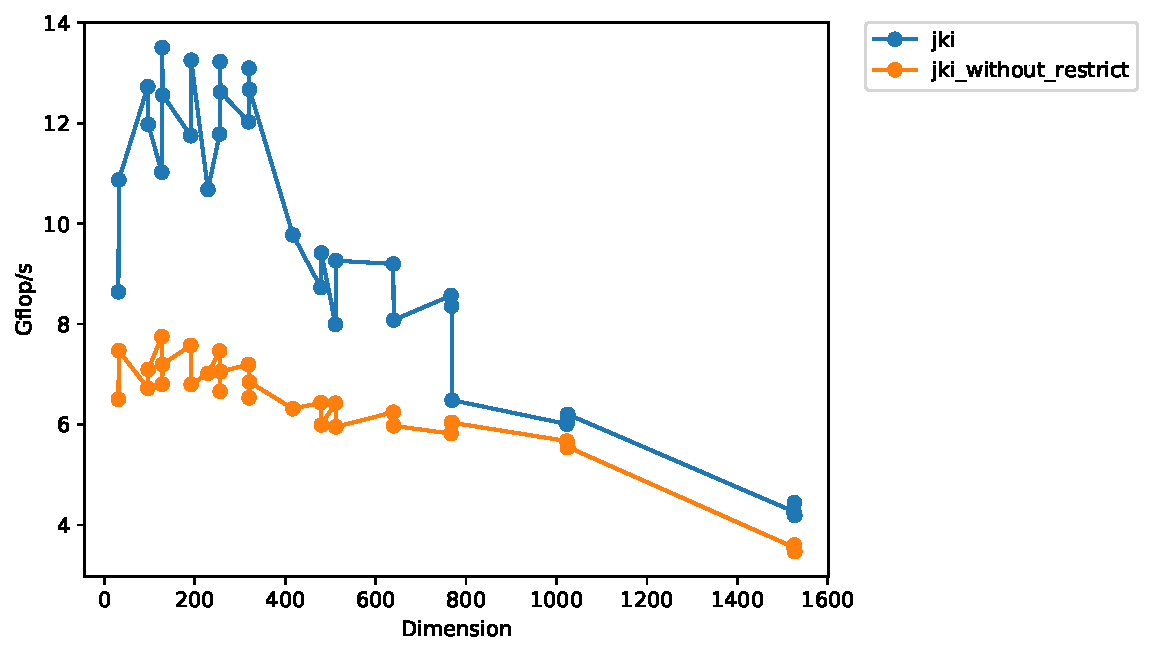
\includegraphics[width=0.8\columnwidth]{timing_jki_restrict.pdf}
    \caption{Flop rates with and without the \texttt{restrict} keyword.}
    \label{fig:Restrict}
\end{figure}



\subsection{Loop Order}
In the basic algorithm, matrix multiplication of two $M\times M$ matrices is performed in a sequence of three nested loops:
\\do i=1,M;	do j=1,M;	do k=1,M
\\ C[i,j]+=A[i,k]*B[k,j]\\
The loop order written as above is ijk.
The sequence of the i, j and k loops does not influence the accuracy of the calculation or the number of individual calculations. However, it has a profound effect on the time required due to the column major storage of arrays. This can be quantitatively observed in figure \ref{fig:LoopOrder}. As the data is stored in the column major format, accessing C is faster if we first loop through the rows of a given column first. Hence, having i loop as the inner most loop is fastest i.e. the plots labelled as jki and kji in figure \ref{fig:LoopOrder}. Same logic applies while accessing the elements of the array B and looping through the rows of B i.e. the k loop before the columns i.e. the j loop is more efficient than vice versa. Hence, jki is faster than kji in figure \ref{fig:LoopOrder}. In the rest of the report jki loop order is assumed.
\begin{figure}[h!]
    \centering
    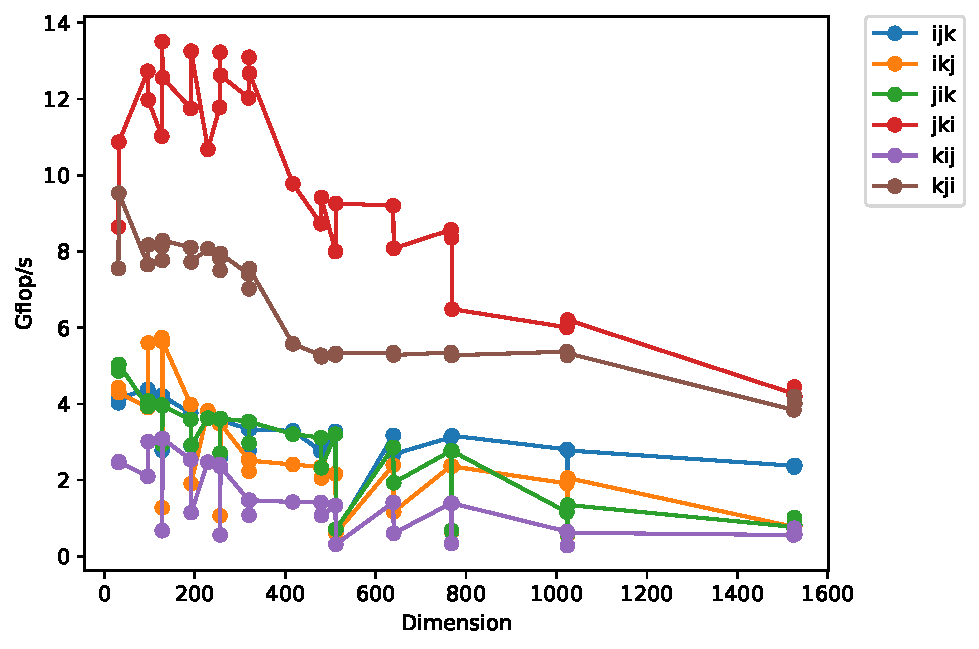
\includegraphics[width=0.8\columnwidth]{timing_loop_order.pdf}
    \caption{Flop rates for each of the six possible loop orders for the kernel.}
    \label{fig:LoopOrder}
\end{figure}

\subsection{Register Allocate}\label{sec:RegisterAllocate}
Considering the jki loop order, the innermost loop reuses B[k,j]. Thus it can be register allocated such that it is fetched from the memory only once. \footnote{\label{Ref1}Lam MD, Rothberg EE, Wolf ME. The cache performance and optimizations of blocked algorithms. ACM SIGOPS Operating Systems Review. 1991 Apr 1;25(Special Issue):63-74.} Practically this implies changing the algorithm to:  
\\do k=1,M;	do k=1,M;	\\r=B[k,j]\\do i=1,M
\\ C[i,j]+=A[i,k]*r\\
The benefit of register allocating is observed for the largest matrix size only in figure \ref{fig:Registering}. For smaller matrices it is sometimes slightly detrimental. This is perhaps because for smaller matrices cache is big enough to hold B[k,j] in the memory by the time it has to be reused and writing it to another variable r reduces performance.\footnotemark[\ref{Ref1}]
\begin{figure}[h!]
	\centering
	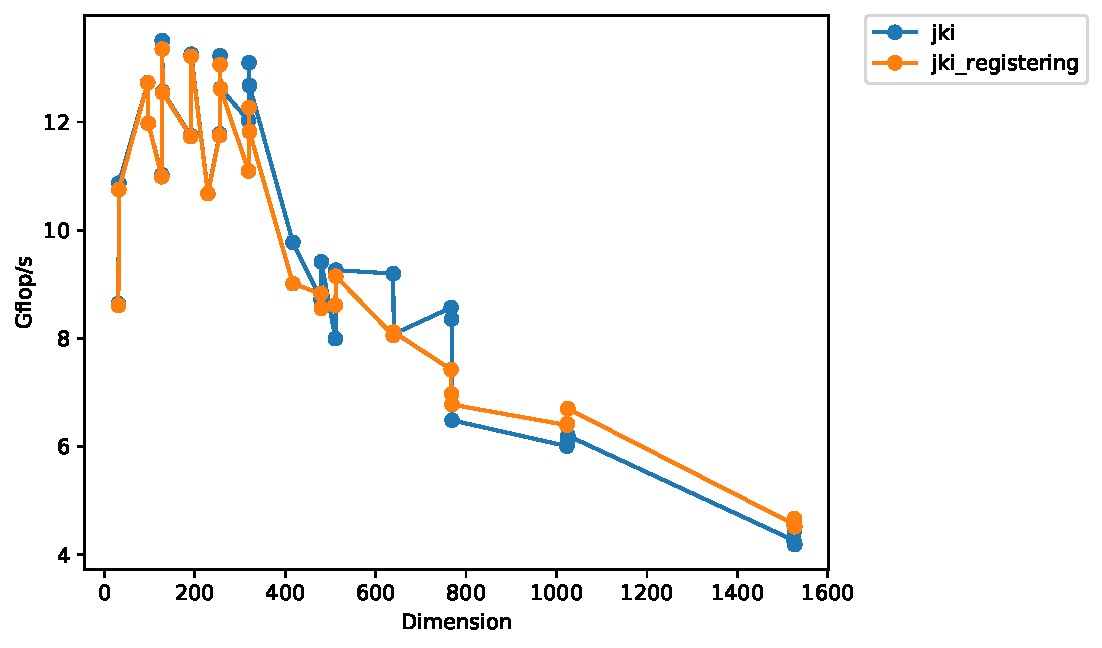
\includegraphics[width=0.8\columnwidth]{timing_jki_registering.pdf}
	\caption{Flop rates with and without register allocating.}
	\label{fig:Registering}
\end{figure}
\section{Discussion: Blocking}

If the calculations are performed on submatrices fetched from the original matrix that can completely fit into a faster level of memory hierachy such as cache, average access latency is reduced and the number of flops in a given time are increased.\footnotemark[\ref{Ref1}] This is the idea behind blocking that allows an improved performance. 

However, block size is a parameter here and can largely affect the performance as observed from figure \ref{fig:Blocking}. Comparing figure \ref{fig:Registering} and \ref{fig:Blocking} we observe that almost all the block sizes tested lead to a better performance. However, the most efficient block size depends upon the size of the matrix. As mentioned by Lam et al. \footnotemark[\ref{Ref1}], the matrix size and cache parameters must be taken into account to obtain a most efficient block size (choosing a block size to fill whole cache or a fixed portion of cache is not the best strategy). While we have not tailored the block size for each dimension, from figure  \ref{fig:Blocking} we can see that blocking with 64 as the block size leads to near optimal performance for all the dimensions considered.

\begin{figure}[h!]
	\centering
	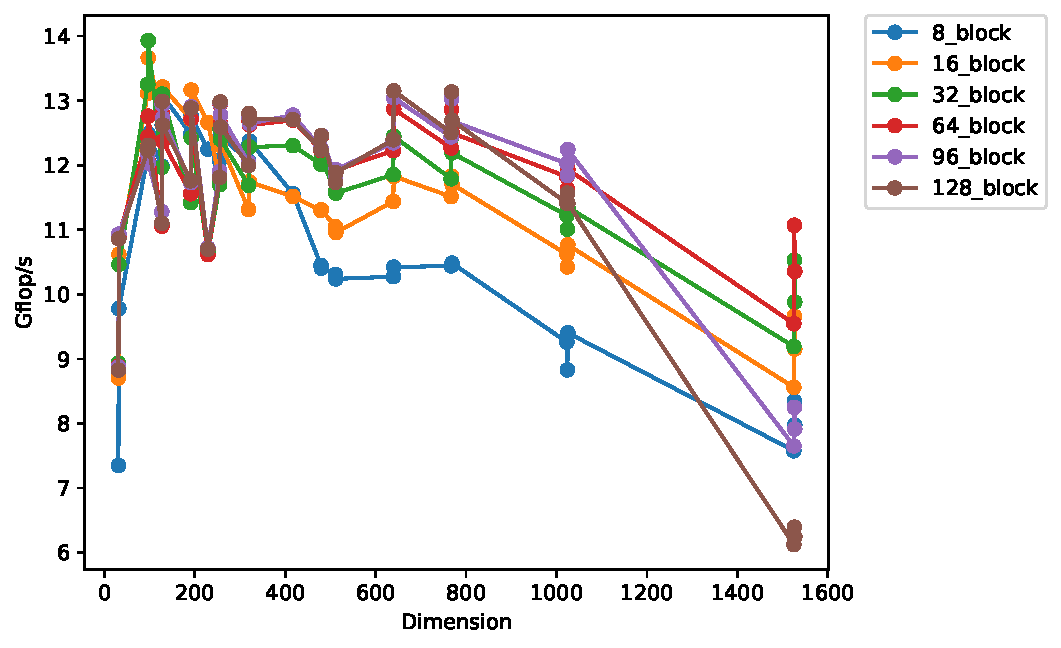
\includegraphics[width=0.8\columnwidth]{timing_block_size.pdf}
	\caption{Flop rates with different block sizes, e.g. 64\_block indicates blocking with a size of 64.}
	\label{fig:Blocking}
\end{figure}

\subsection{Effect of register allocating with blocking}
Figure \ref{fig:BlockingRegistering} shows the effect of register allocating (section \ref{sec:RegisterAllocate}) when combined with blocking with 64 as the block size. The improvement due to register allocating is negligible. Neverthless, we keep register allocation in the final algorithm whose results are reported in figure \ref{fig:timing_methods}.

\begin{figure}[h!]
	\centering
	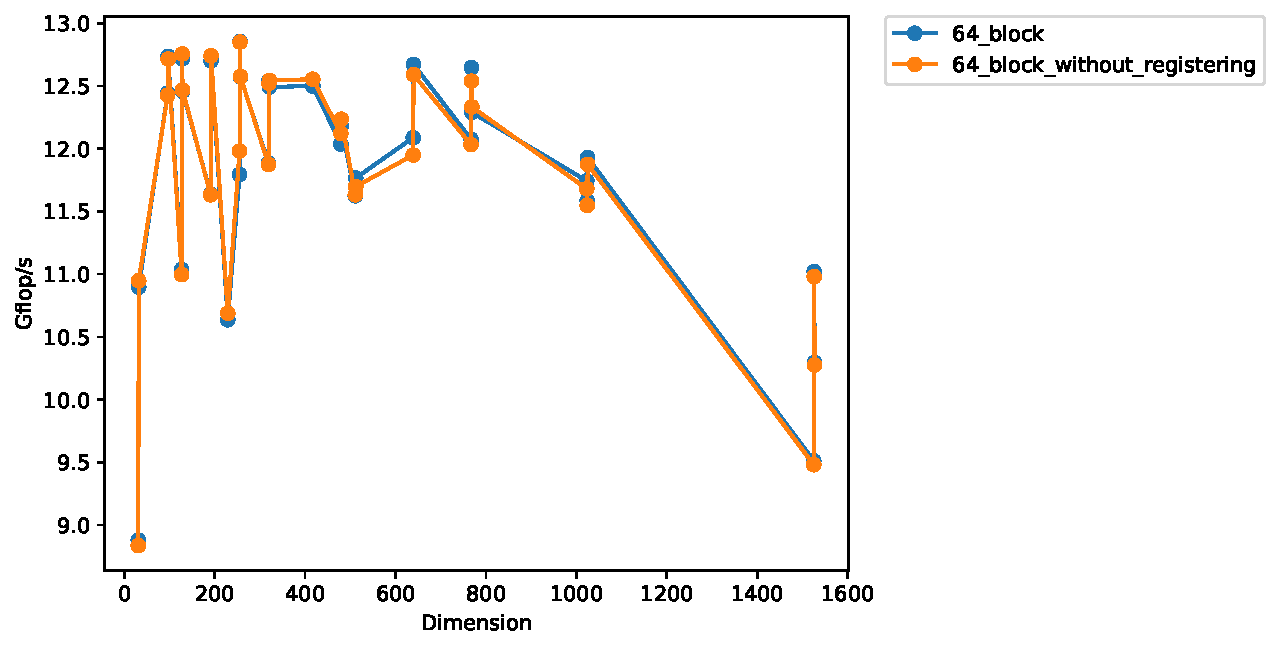
\includegraphics[width=0.8\columnwidth]{timing_64_block_registering.pdf}
	\caption{Flop rates with and without register allocation when combined with blocking with 64 block size.}
	\label{fig:BlockingRegistering}
\end{figure}

\section{Conclusion}

As mentioned in the Introduction we are able to improve upon the basic algorithm by about 3 times. However, we are below BLAS by almost 2.5 times. Three changes provide the most benefit: (a) restricting the .... (b) optimizing the loop order to exploit the memory structure and (c) blocking by performing calculations on sub-matrices that can fit in the cache. Implementation of register allocation has mixed results especially when combined with blocking.

We tried certain other things that have negligible or negative consequence on the performance. These include coping ... First, copying large amounts is bad. For instance, as a form of copy optimization, we attempted to copy the whole of \texttt{A}, \texttt{B}, and \texttt{C} into structured aligned arrays. However, any potential improvement due to alignment was negated by the large amount of time moving memory. With more careful timing and storage, it is likely that alignment could be used to effect, but it would take much more attention to detail than simple copying. Another option would be to use the specific commands allowed by the Intel compiler, shown in the \texttt{kdgemm.c} example.

Second, large improvements in the flop rate could be made with simple changes to the code and compiler. For instance, after the addition of three compiler flags, changing the loop order of the basic code, and adding the \texttt{restrict} keyword, the speed of the code improved by approximately an order of magnitude, especially for small matrices. However, when we tried writing large amounts of code (e.g., when trying the copy optimization previously described), the performance tended to go down. 
\begin{itemize}
	\item We should have more carefully profiled our code. 
	\item Specific details about what is happening on a computer are important.
	\item BLAS is impressive, but weirdly slow for small matrices.
	\item Alignment is confusing
\end{itemize}



\end{document}